\chapter{Background}

This chapter presents a background on the current state of searching lifelog images. This is done through a review of the literature and findings from the NTCIR-12 lifelog semantic access task. 

% ---------------------------------
%  BEGIN LIT REVIEW
% ---------------------------------
\subsection{Representing the Data}
One way of viewing lifelogging is the process of creating a surrogate memory for a person. Organising and presenting are the key challenges for lifelog search engines. Gurrin et al.~\cite{gurrin2014lifelogging} proposes that it is possible to segment the raw, unprocessed lifelog data into meaningful units, or events; which he defines as: "a temporally related sequence of lifelog data over a period of time with a defined beginning and end". In order to perform information retrieval, the events need to be annotated with meaningful semantics. Annotations can either be manually created by humans, or generated through machine learning algorithms. These annotations must also be evaluated for effectiveness, as poor annotations will lead to poor performance when performing retrieval on the images.

There are five aspects of human memory access, as proposed by Gurrin et al.~\cite{gurrin2014lifelogging}:
\begin{enumerate}
    \item Recollecting: Concerned with re-living and accessing past experiences of episodic memories.
    \item Reminiscing: A form of recollecting, concerned with reliving past experiences for emotional or sentimental reasons.
    \item Retrieving: A more specific form of recollecting  in which specific information needs are to be retrieved such as an address, a document, a location, or any atomic piece of information.
    \item Reflecting: A form of quantified-self analysis, performed in order to discover knowledge and insights that may not be immediately obvious.
    \item Remembering: Concerned with prospective memory more than episodic memory. A form of planning for future activities or to act as a reminder or prompt for tasks that a person would like to do.
\end{enumerate}
Gurrin et al.~\cite{gurrin2014lifelogging} argues that an information retrieval system targeted at lifelogging should focus on the Five R's as information needs for the user.

In the context of searching images on the web,  L. Vuurpij, et al.~\cite{vuurpij2002vind} states that image retrieval systems are restricted to the domain they cover and require a lot of domain knowledge in order to fulfil the information needs of a user. Furthermore, L. Vuurpij, et al.~\cite{vuurpij2002vind} notes that there has been a shift from computer vision and pattern recognition to psychology and cognitive science in the domain of image retrieval, where models like the Five R's~\cite{gurrin2014lifelogging}, are becoming more prevalent. 

\subsection{Annotating Lifelog Images}
The current state of the art models for image retrieval use tag-based or textual description annotations \cite{ali2010semantically}. This is typically due to the fact that retrieval models can use this text as a bag of words, or use the text to attribute some form of semantic meaning.

\subsection{Evaluating Annotations}
Without high quality annotations, semantic search would not work, since semantic search exploits the meaning and context of a sentence rather than the keywords in it \cite{ali2010semantically}. The semantic and contextual data associated with images is important for an effective retrieval model that uses textual features rather than pixel data in images. This textual data can either be generated using machine learning algorithms, as demonstrated by A. Karpathy et al.~\cite{karpathy2015deep} and  I. Sutskeve et al.~\cite{sutskever2011generating}, or generated manually by humans. The machine learning algorithms do however start from test data, typically of a specific domain or a range of domains, which they learn from. It is important to note that this can have undesirable consequences when trying to apply a model which has been trained on one domain to one which it has no knowledge of. In both situations, it is essential that the annotations themselves are evaluated such that they describe the image with enough detail and are convincing to humans, since queries will be formulated by humans. Three widely used models for this exist: BLEU \cite{papineni2002bleu} which is precision based, ROUGE (Recall-Oriented Understudy for Gisting Evaluation) \cite{lin2004rouge} which is recall based, and METEOR \cite{elliott2013image}, used for judging the overall quality of annotations.

All of the metrics above were initially proposed with respect to the evaluation of automatic summarisation and natural language processing. Furthermore, they all use a reference annotation in order to score annotations. ROUGE compares the number of overlapping n-grams, word sequences, and word pairs of annotations with ideal annotations created by humans \cite{lin2004rouge}. BLEU counts the maximum number of times a word appears in any reference annotation, followed by "clipping" the total count of each candidate word by its maximum reference count, adding these "clips" up, and dividing by the total unclipped number of candidate words in the annotation \cite{papineni2002bleu}. The notion of "clipping" in BLEU is a variation of precision whereby words are only accepted for the maximum number of times they appear the reference text, for instance if a word appears in an annotation five times but is in the reference annotation twice, the "clipped" value would be 2/5. Finally, METEOR generally operates by unigram matching (bag of words) between a reference annotation, typically created by a machine, and a human produced annotation. Both METEOR and ROUGE take multiple approaches to comparing annotations, for reference, ROUGE:
\begin{enumerate}
    \item ROUGE-N N-gram Co-occurence Statistics
    \item ROUGE-L Longest Common Subsequence
    \item ROUGE-W Weighted Longest Common Subsequence
    \item ROUGE-S Skip-Bigram Co-Occurence Statistics
    \item ROUGE-SU Skip-Bigram Co-Occurence Statistics with Unigram\\ Counting Unit
\end{enumerate}
The unigrams matched in METEOR can be based on surface forms, stemmed forms, and meanings, with the option to be extended \cite{elliott2013image}.

R. Vedantam et al.~\cite{vedantam2015cider} argue through the results of their experimentation, however, that there exists a more effective model for evaluation which is rooted in human consensus. Their method, CIDEr (Concensus-based Image Description Evaluation) is a model which outperforms all other models of evaluating descriptive annotations of images. CIDEr performs so well due to high correlation with human judgement and consensus. According to R. Vedantam et al.~\cite{vedantam2015cider}, the CIDEr metric inherently captures sentence similarity, the notions of grammatically, salience, importance (precision), and accuracy (recall). CIDEr appears to improve upon the other three models and takes into account the weaknesses the other models may have, however it still relies on reference annotations.

The evaluation methods above rely on the availability of a ground truth or reference annotation that can be used to compare with the automatically generated annotation. This approach, however, is ill-suited to generating annotations for lifelog images as it is unclear what these annotations should ``look like'', because it is unknown what makes an annotation of a lifelog image ``good''. A better suited alternative for this problem is to embed the evaluation of different annotation methods within a task and thus evaluate the  methods with respect to the effectiveness the different methods induce on the task. Specifically, in this research project, the aim is to embed the evaluation of lifelog annotation within a search task. Thus the effectiveness of a system would be evaluated with respect to the search task. None of the system properties would vary apart from the method that is used to annotate images.This evaluation methodology is akin to, for example, previous work that has examined the effectiveness and quality of different topic modelling techniques and semantic models via evaluating the effect they have on search engine result effectiveness~\cite{wei2006lda,zuccon2015integrating,karimzadehgan2010estimation,yi2009comparative}.

\subsection{Types of Annotations}
As suggested by R. Yan et al.~\cite{yan2008learning}, the most common image annotation approaches can be categorised into two types. The first is \textit{tagging}, where annotators choose a set of keywords from a vocabulary for each image. The second most common approach is described as \textit{browsing}, where a group of images are judged against the relevance of a predefined keyword. There are, however, less commonly used annotation approaches, for example, \textit{descriptive natural language annotations} which are generated in a model by A. Karpathy et al.~\cite{karpathy2015deep}. This model outperforms the previous work done in this area of research for both image retrieval and image annotation on the Flickr8K, Flickr300K and MSCOCO. B. Hu et al.~\cite{hu2003ontology} clarifies why high quality textual descriptions generally perform better than systems that employ keyword or tag based annotation models, in that these models suffer from several limitations:
\begin{enumerate}
    \item A keyword in a document does not necessarily mean that the document is relevant
    \item A relevant document may not contain the explicit word
    \item Synonyms of the query keywords lower the recall rate (ratio of retrieved images which are relevant to the total number of relevant images, see Appendix A for details)
    \item Homonyms of the query keywords lower the precision rate  (ratio of relevant images that are successfully retrieved to the total number of relevant and irrelevant images retrieved) see Appendix A for details)
    \item Semantic relations such as hyponymy, meronymy, antonymy are not exploited
\end{enumerate}

Recent work in the consumer health search domain by Zuccon et al.~\cite{quteprints82599} and Stanton et al.~\cite{stanton2014circumlocution} focused on generating queries from images. The aim of their research was to understand how the general public would search for information if they had a medical condition as that in the image presented to them. This new methodology used by these previous works could be adapted to the context of gathering annotations for lifelogging, thus leading to an \textit{annotation by querying} method. This method would consist of showing annotators an image from a lifelogger and ask them to provide the queries they would issue to a (standard) search engine to attempt to retrieve the image itself.

\subsection{Searching for Lifelog Images}
Lifelog information retrieval systems typically have very poor performance due to there not being any formal models made specifically for the field, as reported by Gurrin et al.~\cite{gurrin2014lifelogging}. Until very recently, there have been no large, distributable test collections such as the TREC collection for text \cite{gurrin2014lifelogging}. The NTCIR collection is a set of tagged lifelog images which have been collected by researchers who wore a lifelogging camera for a short amount of time \cite{gurrin2016ntcir}. The tags were automatically generated by using a pre-trained image tagging algorithm.

While there is limited applied methodology to retrieval models in lifelogging, there has been much discussion about what the models should try and solve. Both H.  W.  Bristow et al.~\cite{bristow2004defining} and A. R. Doherty et al.~\cite{doherty2010automatically} corroborate that detecting and interpreting the implicit semantics and context of lifelogging data from heterogeneous sources would be advantageous in explaining the Who?, What?, Where? and When? questions which occur in every day events. It was also noted that these questions are common among image searchers and that they are not capable of being answered by normal indexing like that in traditional search engines \cite{ali2010semantically}.

While there has been some research into tagging and annotating images, there has not been as much work in developing a model for searching these images within the context of lifelogging \cite{gurrin2014lifelogging}. Typical image search engines for web pages treat the surrounding text, captions, alternate text and HTML titles \cite{frankel1996webseer} as a bag of words for retrieval. The success of these search engines rely on a sufficient amount of surrounding text, something which is not provided by current automatic image annotation models for lifelogging. The longer and more detailed the text is within the context of the image, the better the performance of the search engine. This is perhaps why other research has involved novel search techniques \cite{vuurpij2002vind}, since the current models for generating captions of images are not yet detailed or accurate enough for current textual information retrieval models to work.

Generally, image based retrieval methods can be classified into two categories: text-based image retrieval (TBIR) and content-based image retrieval (CBIR). A CBIR system utilises image features such as grid colour movements, edge direction histogram, Gabor textual features, and Local binary pattern histograms. as described in work by Wu et al.\cite{wu2009distance}. These features (colour, texture, shape, SIFT keypoints) become a query to the search engine which match visually similar images. CBIR systems, although extensively studied for over a decade, are still limited in comparison to TBIR systems. Zue et al.\cite{zhu2010image} provide three points for why this is:
\begin{enumerate}
    \item The semantic gap that exists between low-level visual features and high-level semantic concepts
    \item The low efficiency due to high dimensionality of feature vectors
    \item The query form is unnatural for image searching (appropriate example images may be absent)
\end{enumerate}
The efficiency of TBIR can be explained when one considers that it can be formulated as a document retrieval problem and can be implemented using the inverted index technique. The downside to TBIR is that is highly expensive: experimental evidence by Wu et al.~\cite{wu2013tag} shows that the performance of TBIR is highly dependent on the availability and quality of manual annotations. If this process can be automated and images can be automatically captioned, it would solve a fundamental issue that exists with TBIR systems.

\subsection{Automatically Captioning Images}

There have been some recent advances in machine learning which combine convolutional neural networks and recurrent neural networks that enable images to be automatically captioned. This elegant recipe of feeding the last hidden layer of the CNN as input into the RNN is followed by current state of the art automatic image captioning systems such as those of Karpathy et al.~\cite{karpathy2015deep} and Vinyals et al.~\cite{arXiv2016160906647V}.

Generating captions for images reduces the expensiveness of TBIR systems, although manually annotating or labelling a test collection still takes time. This process may be able to be alleviated by automatically generating images from text. Recent machine learning architectures like that of Reed et al.~\cite{reed2016generative}, while limited to specific domains, can produce images from textual descriptions. In time this could allow hybrid TBIR/CBIR systems that outperform the current state of the art image retrieval systems.

% ---------------------------------
%  END LIT REVIEW
% ---------------------------------

\section{Findings From NTCIR}
The NTCIR-12 lifelogging latent semantic access pilot task consists of four research teams contributing to the automatic retrieval component and one participant in the interactive retrieval component. The highest performing automatic team, LIG-MRIM, uses computer vision to classify images and does not rely on the visual concepts distributed with the task. The interactive team (LEMoRe) outperformed all other automatic teams, but this is generally the case with tasks that contain both automatic and interactive components. The three other automatic teams are consisted of VTIR, III\&CYUT and QUT (the preliminary work done for this research).

LIG-MRIM~\cite{safadilig2016ligmrim} uses dynamic convolutional neural networks and a multi-class support vector machine (MSVM) in order to classify images. Visual indexing is composed of two parts: three deep convolutional neural network models (AlexNet, GoogleNet and Visual Geometry Grouping (VGG)) process each image. The output is normalised and has principal component analysis (PCA) performed on it. These outputs are then concatenated together. The same normalisation and PCA process is repeated and fed into the MSVM. The output of this is concatenated with the VGG data. The second part involves temporally naming times of the day in order to attempt to extract semantic meaning from times of the day. While this team submitted runs that fit the definition of automatic for the task, queries were generated manually from the topics by an expert.

The VTIR team~\cite{xia2016vtir} attempts to exploit location meta data associated with the images. To this end 3,000 random images are labelled against a rich semantic location ontology. More concepts are utilised by applying the WordNet database to find cognitive synonyms. Despite the additional annotations, this system failed to provide good retrieval effectiveness.

III\&CYUT~\cite{lin2016image} uses a traditional textual based approach to lifelog retrieval. A skipgram word embedding obtained with word2vec\cite{mikolov2013word2vec} is computed for the visual concepts distributed with the data set. These embeddings are then used in an attempt to add more semantic meaning to images. Specifically, the embeddings are used within a document expansion process, resulting in a translation language model~\cite{zuccon2015integrating}. Query expansion is also used on every keyword.

The QUT team~\cite{scells2016qut} manually annotates a subset of the images in the collection with long textual descriptions. To select images for annotation, they follow an approach based on temporal and visual clustering of the images. They then further extend the annotation process by propagating the annotations to other images contained within the same cluster of already annotated images.

Finally, the LEMoRe~\cite{de40lemore} team, which use an interactive approach, combine existing technologies and methodologies in order to develop a search engine. Colour correlogram, edge histogram, joint composite descriptor and pyramid histogram of oriented graphics are used by the image retrieval system as features to retrieve images. Both a novice and an expert used the system to produce runs.

The results from this pilot task offer a promising glimpse into the future of searching lifelog images. Figure \ref{fig:ntcir-results} presents the best run from each of the teams that participated in NTCIR-12 LSAT. LIG-MRIM shows that automatic methods for annotating lifelog images can result in decent text-based image retrieval effectiveness. The teams that do not perform well (including the QUT team) offer insight into areas of research to avoid. 

The difference in retrieval effectiveness between LIG-MRIM and the other three teams is highly likely due to the annotations of the images. The task provides teams with automatically generated annotations for the images distributed with the task. These annotations are generated using a previously state-of-the-art captioning framework, CAFFE~\cite{jia2014caffe}. The problem lies within the fact that a CAFFE model is trained on a data set that does not align with the lifelog images. Three of the teams use these annotations in their systems; however LIG-MRIM generate their own annotations. This indicates that no matter how well tuned and suited a text-based image retrieval system is to lifelog images, poor textual representations for images can significantly impact the retrieval effectiveness.

\begin{figure}[hb]
    \centering
    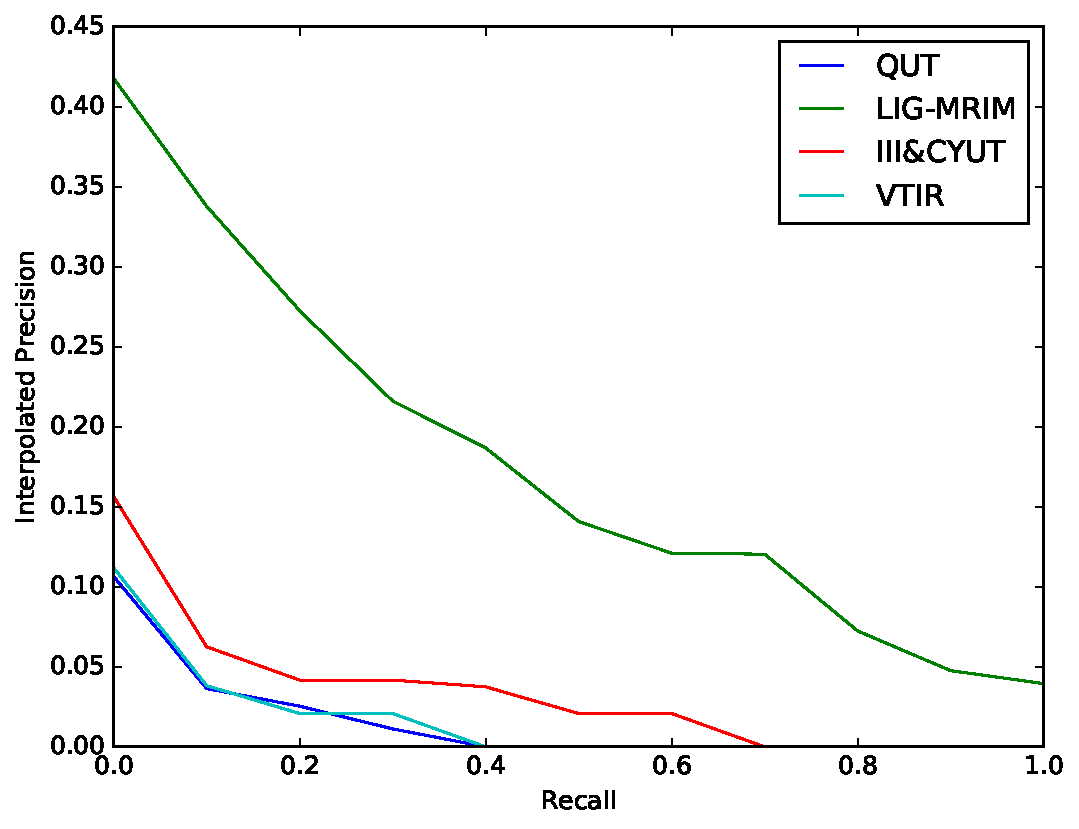
\includegraphics[width=0.95\textwidth]{graphs/ntcir-pr-curve}
    \caption{Precision-recall curves for the four LSAT teams}
    \label{fig:ntcir-results}
\end{figure}